\documentclass[12pt,a4paper]{article}
\usepackage[utf8]{inputenc}
\usepackage{graphicx}
\usepackage{hyperref}
\usepackage{geometry}
\geometry{margin=2.5cm}

\title{\textbf{MLLB Report: Machine Learning Pipeline Development}\\ \large Machine Learning for Big Data}
\author{Nicolas CASTEL}
\date{\today}

\begin{document}
\maketitle

\section{Introduction and MLOps Methodology}
This report details the practical implementation of machine learning pipelines using Python and \texttt{scikit-learn}. The project adheres to MLOps best practices by separating the exploratory analysis (Jupyter Notebooks) from the reusable preprocessing pipelines (\texttt{src/preprocessing.py}) and maintaining version control via Git and GitHub.

\section{Exploratory Data Analysis Implementation}
The initial Exploratory Data Analysis (EDA) was performed using \texttt{pandas} for data manipulation and \texttt{seaborn}/\texttt{matplotlib} for visualization. A correlation heatmap was generated using \texttt{sns.heatmap()} to inspect relationships between weather variables and hourly bike rentals, directly informing our feature selection process.

\section{Data Preprocessing and Feature Engineering}
To ensure code reusability, a custom Python module (\texttt{src/preprocessing.py}) was developed. The \texttt{load\_and\_preprocess()} function programmatically executes the following:
\begin{itemize}
    \item \textbf{Data Leakage Prevention:} Features that sum up to the target (\texttt{casual}, \texttt{registered}) were dropped.
    \item \textbf{Redundancy Removal:} Highly correlated features such as \texttt{atemp} were removed to streamline the pipeline.
    \item \textbf{Target Engineering:} A binary target variable, \texttt{is\_peak\_demand}, was engineered using the 75th percentile of the rentals to prepare for the subsequent classification task.
\end{itemize}
Features were subsequently scaled using \texttt{scikit-learn}'s \texttt{StandardScaler} to normalize the data distributions for distance-based and regularized models.

\section{Regression Implementation and Tuning}
The regression task aimed to predict total hourly rentals (\texttt{cnt}). Two models were implemented and evaluated using RMSE, MAE, and $R^2$ metrics:
\begin{enumerate}
    \item \textbf{Baseline:} A standard \texttt{LinearRegression()} estimator was fitted, providing a computational baseline.
    \item \textbf{Ensemble Model:} A \texttt{RandomForestRegressor()} was implemented. To optimize the ensemble, \texttt{RandomizedSearchCV} was utilized to efficiently sample the hyperparameter space (tuning \texttt{n\_estimators} and \texttt{max\_depth} across 3 folds).
\end{enumerate}

The optimized Random Forest significantly outperformed the baseline. A scatter plot comparing true vs. predicted values was generated and saved programmatically to visualize the model's accuracy (see Figure \ref{fig:regression_results}).

\begin{figure}[h]
    \centering
    % 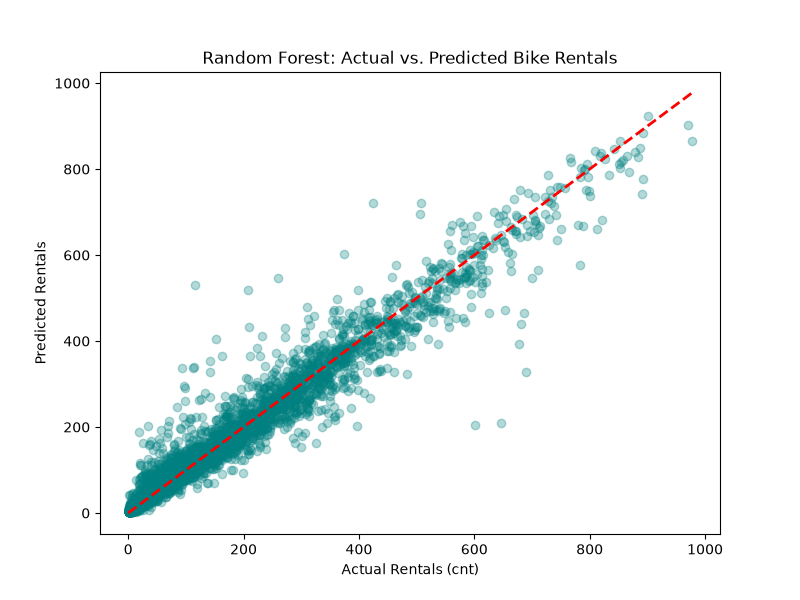
\includegraphics[width=0.8\textwidth]{../figures/rf_regression_results.png}
    \caption{Random Forest Predictions vs. Actual Rentals (Placeholder)}
    \label{fig:regression_results}
\end{figure}

\section{Classification Implementation}
% To be completed: Implementation of tree-based models vs linear models, and confusion matrix plotting.

\section{Unsupervised Implementation}
% To be completed: Scikit-learn implementation of PCA and K-Means, including Elbow method plots.

\section{AI Assistants and Copilot Integration}
GitHub Copilot was integrated into the VS Code environment to assist with pipeline generation. Copilot was specifically prompted to write the cross-validation logic using \texttt{RandomizedSearchCV}, accelerating the hyperparameter tuning phase. All AI interactions and generated code were reviewed for syntactical correctness and logical validity.

\end{document}